\begin{savequote}[75mm]
The outcome of any serious research can only be to make two questions grow where only one grew before.
\qauthor{Thorstein Veblen}
\end{savequote}

%For an example of a full page figure, see Fig.~\ref{fig:myFullPageFigure}.

\chapter{Video Segmentation by Relaxation of Tracked Masks}
\label{Chap:VideoSegRelaxation}
\lettrine[lines=3, loversize=0.3]{\textcolor{DarkBlue}I}{n the beginning}, 3D data, especially video data, was not readily available. As such, researchers were forced to make due with strictly 2D video, which is inherently ambiguous in many situations. In particular, partial and full occlusions are particularly vexing problems in 2D video - not least because understanding of 2D video is so easy for humans, yet so difficult to interpret algorithmically. Indeed, knowledge of object permanence, that is, the understanding of how to correctly interpret occlusions, is something that humans acquire very early on in their lives \cite{ObjectPermanence}, but has yet to be successfully implemented in a fully automated \gls{vos} system. Even after decades of research, state-of-the-art methods still have trouble correctly resolving partial occlusions, and typically fail completely after even the briefest of complete occlusions.

In this Chapter, we shall present our attempts towards resolving the object permanence problem with 2D data, as well as advance color-based \gls{vos} in general. In particular, we seek to overcome two of the main drawbacks of the color-based video segmentation method developed by Abramov et al. \cite{Abramov_RealtimeSegmentation} (and indeed, of color-based \gls{vos} in general). The first of these is the correct tracking of objects through partial and full occlusions, which we proposed to solve using a layering of deformable object masks that are allowed to interact and compete for ``ownership'' of pixels. The second is to allow for object identities to be maintained through sudden and/or fast movements - something that was not possible due to the core assumptions of the algorithm. To correct for this, we tracked the masks with a set of particle filters, a class of Bayesian predictive filters which are well known for their ability to handle difficult trajectories \cite{TrackingMultipleParticleFiltering,MonteCarloMTT,SequentialMonteCarloMultitargetFiltering}.

The underlying principle guiding the proposed algorithm is to use predictions from Bayesian filtering to inform segmentation of higher-level temporal object correspondences. It is well known that sequential Bayesian estimation methods perform well in difficult tracking scenarios \cite{Doucet2001}, and, under the Markov assumption, are computationally less demanding than video segmentation techniques such as MHVS \cite{MHVS}, which consider many prior frames. Particle filtering is one such method which has been shown to approximate the optimal tracking solution well, even in complex multi-target scenarios with strong nonlinearities \cite{TrackingMultipleParticleFiltering,MonteCarloMTT,SequentialMonteCarloMultitargetFiltering}. 

\section{Overview of the Algorithm}
\label{sec:Overview}
Before proceeding to discuss elements in detail, we shall first give a brief overview of the algorithm (depicted in Figure \ref{fig:AlgorithmFlow}). We begin by performing an initial segmentation (using any method) on the first frame $\mathbf{F}_{t_0}$ to generate an initial set of labels $\mathbf{S}_{t_0}$. An initial set of particles is generated for each label, and color histogram features are computed for each particle (as in \cite{ColorBasedProbabilisticTracking}). Thus each object $k$ at initial time $t_0$ is specified by a set of $N_k$ particles $\mathbf{X}^{k,1:N_k}_{t_0}$, each of which contains a representation of the object, specified by a pixel existence map $\mathbf{M}$, a reference color histogram $\mathit{\hat{q}}$, a position shift vector $\mathbf{p_{t_0}}$, and a velocity vector $\mathbf{v_{t_0}}$.

\begin{figure}[!t]
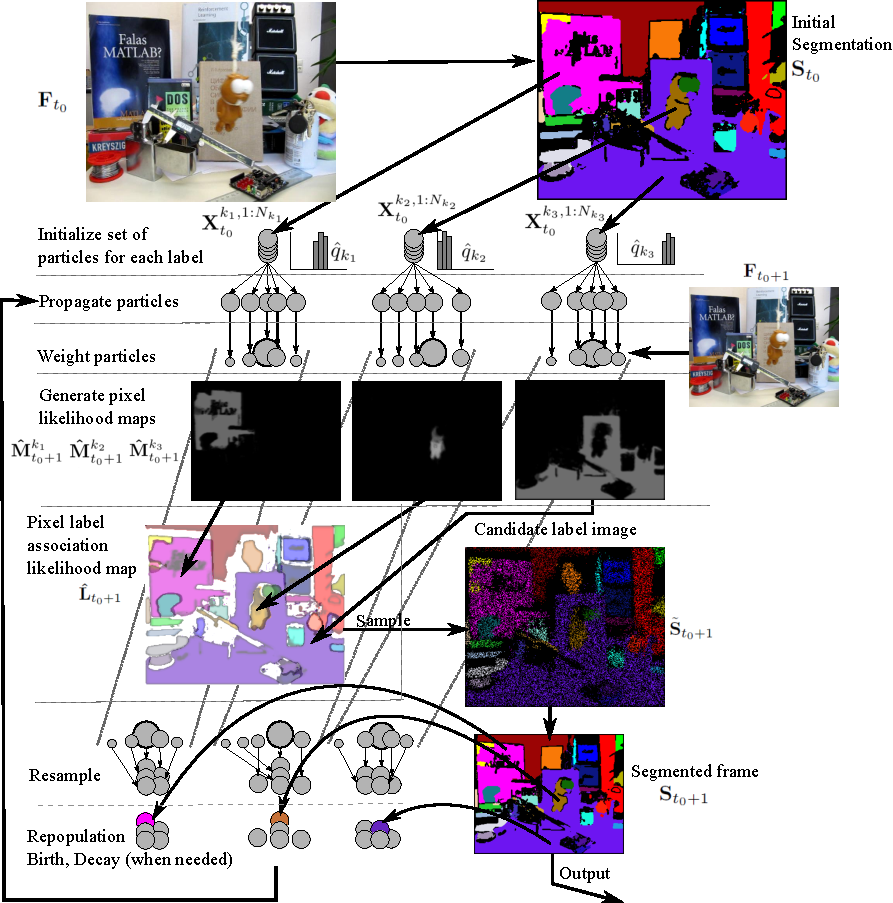
\includegraphics[width=\linewidth]{figures/ECCV2012/AlgorithmFlow2.pdf}
  \caption[Overview of Algorithm]{Flow of algorithm for one time step, shown for three labels ($k_1$, $k_2$, and $k_3$). For a description, see Section~\ref{sec:Overview}.}
\label{fig:AlgorithmFlow}
\end{figure}

The particles are then propagated in time independently, shifting their existence maps to new regions of the image. These shifted maps are used to generate measured color histograms from the next frame, which are evaluated to determine similarity to the object's reference histogram. The set of particles for each object is then combined to create an overall object pixel likelihood map. The pixel likelihood maps for all objects are then further combined with each other to create a label association likelihood map. In this likelihood map, each pixel is a \gls{pdf} specifying the probability that the original image pixel was generated from an observation of a particular object.

The label association likelihood map is then sampled using a per-pixel selection procedure (as described in Section~\ref{sec:LabelAssocLikelihoodMap}) to generate a candidate label image, $\tilde{\mathbf{S}}_{t_0+1}$. This candidate image is used as the initialization for the Metropolis-Hastings algorithm with annealing of Abramov et al. \cite{Abramov_RealtimeSegmentation}, which updates the labels iteratively until an equilibrium segmented state is reached. The segmentation result, $\mathbf{S}_{t_0+1}$  is subsequently used to update the set of particles via three mechanisms; birth, decay, and repopulation. Birth is used for new labels in the segmentation output, and consists of initializing a new set of particles. Decay occurs when a label is not found in the segmentation output, and consists of killing a number of the particles of the missing label. The most commonly occurring mechanism, repopulation, occurs for all previously existing object labels which are found. Repopulation rejuvenates the set of particles for an object by replacing a number of particles in the set with new particles based on the relaxed segmentation result. 

\section{Tracking Object Masks}
We shall now describe each of the parts of the algorithm given above in further detail, beginning with a description of how we track object masks using particle filters. First we will briefly review the basic principles of sequential Bayesian estimation and particle filtering, and then show how they can be used to predict pixel-level label associations in order to seed a segmentation algorithm.

\subsection{Sequential Bayesian Estimation}
Sequential Bayesian estimation uses a state space representation, in which a state vector $\mathbf{x}_t$ describes the hidden state of a dynamic system. Bayesian estimation attempts to determine the posterior distribution of the state given all prior observations $\mathbf{z}$, i.e., $\mathit{p}(\mathbf{x}_t|\mathbf{z}_{1:t})$. This is accomplished using a two step recursion which first generates a hypothesis of the current state conditioned on the previous state and then performs a Bayes update using the new observation. These steps are known as the prediction and filtering steps, respectively. 

The prediction step estimates the current distribution given all prior observations, or
\begin{equation} \label{eqn:prior}
\mathit{p}(\mathbf{x}_t|\mathbf{z}_{1:t-1}) =  \int{ \mathit{p}(\mathbf{x}_t|\mathbf{x}_{t-1})\mathit{p}(\mathbf{x}_{t-1}|\mathbf{z}_{1:t-1}) \mathit{d}\mathbf{x}_{t-1}}. 
\end{equation}
This prediction requires the specification of a stochastic \textit{dynamic model} 
\begin{equation} 
\mathbf{x}_t = \mathit{f}_t(\mathbf{x}_{t-1},\mathbf{v}_t) ,
\end{equation}
where $\mathbf{v}_t$ is the process noise, which characterizes the state transition density $\mathit{p}(\mathbf{x}_t|\mathbf{x}_{t-1})$. The dynamic model takes advantage of knowledge of the system to generate reliable predictions of how the state evolves. 

The filtering step uses Bayes rule to update the predicted density by conditioning it on the new observation $\mathbf{z}_t$:
\begin{equation} \label{eqn:posterior}
\mathit{p}(\mathbf{x}_t|\mathbf{z}_{1:t}) =  \frac{ \mathit{p}(\mathbf{z}_t|\mathbf{x}_{t})\mathit{p}(\mathbf{x}_{t}|\mathbf{z}_{1:t-1})} {\mathit{p}(\mathbf{z}_{t}|\mathbf{z}_{1:t-1})}. 
\end{equation}
This requires the specification of an observation, or measurement, model
\begin{equation} 
\mathbf{z}_t = \mathit{h}_t(\mathbf{x}_{t},\mathbf{w}_t) ,
\end{equation}
where $\mathbf{w}_t$ is the measurement noise, which characterizes the observation density $\mathit{p}(\mathbf{z}_t|\mathbf{x}_{t})$. Once the filtered, or posterior distribution is determined, an estimate of the state can be made using a variety of techniques (e.g., maximum a-posteriori, mean-shift). 

\subsubsection{Dynamic Model}
In our method, the state of a particle consists of four elements; the pixel existence map $\mathbf{M}$, a reference color histogram $\hat{q}$, a position shift vector $\mathbf{p}$, and a velocity vector $\mathbf{v}_t$. Of these, only the position shift and velocity evolve over time, so we adopt the state vector
 \begin{equation} 
 \mathbf{x}_t = [p_x v_x p_y v_y]^T ,
 \end{equation}
where $(p_x,p_y)$ denotes the accumulated shift of the pixel existence map in the image plane, and $(v_x,v_y)$ the map velocity in the image plane. Motion is modeled using a constant velocity model in discrete time with uniform sampling period $\mathit{T}$, giving the dynamic model
\begin{equation} \mathbf{x}_t = \mathbf{A}\mathbf{x}_{t-1} + \mathbf{v}_t , \end{equation}
where
\begin{equation} \mathbf{A} = 
\begin{bmatrix}
 1 & \mathit{T} & 0  & 0 \\ 
 0 & 1 & 0 & 0\\ 
 0 & 0 & 1 & \mathit{T}\\ 
 0 & 0 & 0 & 1
\end{bmatrix} \end{equation}
and noise $\mathbf{v}_t$ is assumed to be zero mean Gaussian with fixed covariance.

\subsubsection{Measurement Model}
In our method measurements are taken by calculating a color histogram, $\mathit{q}_t$ for the region lying within the shifted pixel existence map $\mathbf{M}$. That is, for particle $n$ of object $k$,
\begin{equation}
\mathit{q}^{k,n}_t = hist( \mathbf{F}_{t} \cap \mathbf{M}^{k,n}_t ).
\end{equation}
Color histograms are three dimensional, with 8 bins for each of the color components hue, saturation, and value. As in \cite{ColorBasedProbabilisticTracking}, a Gaussian density is used for the observation density $\mathit{p}(\mathbf{z}_t|\mathbf{x}_{t})$, that is
\begin{equation} 
\label{eqn:Weighting}
\mathit{p}(\mathbf{z}_t|\mathbf{x}_{t}) = \frac{1}{\sqrt{2\pi}\sigma} \exp{-\frac{\Delta(\hat{\mathit{q}},\mathit{q}_t)^2}{2\sigma^2}}, 
\end{equation}
where $\Delta(\mathit{\hat{q}},\mathit{q}_t)$ is the Bhattacharyya distance (as proposed in \cite{Real-timeTrackingMeanShift}) between the reference histogram $\mathit{\hat{q}}$ for the particle and the measured histogram $\mathit{q}_t$ for time $\mathit{t}$. The Bhattacharyya distance is a standard measure of similarity between discrete probability distributions, and is defined as
\begin{equation} \Delta(\hat{\mathit{q}},\mathit{q}_t) = \sqrt{1- \sum{\sqrt{\hat{\mathit{q}}\mathit{q}_t }}}. \end{equation}

\subsection{Parallel Particle Filters}
Except in special cases (e.g., Kalman Filter), closed-form solutions to Equations \eqref{eqn:prior} and \eqref{eqn:posterior} are not available. Particle Filters are a Monte-Carlo method designed to approximate the posterior distribution with a weighted set of random samples. There are many excellent descriptions of the mechanics of particle filtering available (such as \cite{Doucet2001}), so we shall avoid presenting them here, and proceed directly to presenting the details of our algorithm. 

The predictive portion of the method uses multiple Sequential Importance Resampling (SIR) filters in parallel to track multiple targets (labels) simultaneously. At this stage in the algorithm targets are assumed independent and interaction between labels is therefore not considered (interaction is accounted for later, as described in Section \ref{sec:Label Image Generation}). Particles are first propagated using the constant velocity dynamics model, and their predicted existence maps $\tilde{\mathbf{M}}^{k,n}$ are used to generate a measured histogram, $\mathit{q}_t$. Particles are weighted based on \eqref{eqn:Weighting}, and then normalized as a set for each label $k$. Systematic resampling is used to prevent particle degeneracy, due to its speed and good empirical performance \cite{Doucet2001}.

The resulting distributions from the weighting procedure are used to generate object pixel likelihood maps for each label,$\hat{\mathbf{M}}^{k}_{t+1}$, which are then combined into the label association likelihood map $\hat{\mathbf{L}}_t$, as described in Section \ref{sec:Label Image Generation}. A realization of this likelihood map can then be relaxed to produce a final segmented output, $\mathbf{S}_t$. 

\subsection{Particle Birth, Repopulation, \& Decay.}
One key improvement of the proposed algorithm over prior particle filtering methods is its use of the segmentation result $\mathbf{S}_{t}$ to update the particle sets. This allows the creation of new targets, adaptation to changing target appearance, and gradual elimination of targets which are no longer observed. This is accomplished via three mechanisms, which we term, respectively, birth, repopulation, and decay. 

Birth occurs when a label which has not existed previously is found in the segmentation output $\mathbf{S}_{t}$, or more formally $ \{ k\notin \mathbf{S}_{1:t-1}, k\in \mathbf{S}_{t}\}$. It consists of generating a set of particles $\mathbf{X}^k$ for the new label using $\mathbf{S}_{t}$ to initialize an existence map $\mathbf{M}^k_t$ and $\{\mathbf{F}_{t} \cap \mathbf{M}^k_t \}$ to calculate a reference color histogram $\hat{\mathit{q}^k_t}$.

Repopulation is a key component of the algorithm, as it allows the pixel likelihood map for an object, $\mathbf{\hat{M}}^k$, to adapt over time to the changing appearance of the object. Every iteration, all previously existing object labels which are found in $\mathbf{S}_{t}$ are repopulated by replacing some particles in the set with particles generated from $\mathbf{S}_{t}$ and $\mathbf{F}_{t}$. Particles are chosen for replacement using stratified sampling, at a rate specified by parameter $\lambda_r$. The repopulation mechanism gradually modifies the object "model" through the addition of particles which have an updated existence map and color histogram (coming from the segmentation result). We use the term model here loosely, since there is in actuality no explicit model for any of the objects - merely a pixel likelihood map generated at each time step from the objects constituent particles and the current image frame. 

Stratified replacement and relatively low repopulation rates are used to help keep the influence of erroneous hypotheses to a minimum, but as with any adaptive method, they can occasionally lead the tracker astray. Replacement of particles, rather than updating of a central model, helps to reduce this problem, since a few erroneous particles will generally not completely derail the algorithm. Nevertheless, future work could investigate strategies that allow pruning of unlikely hypotheses without negatively affecting occlusion handling. 

Decay occurs when a label is not found in the segmentation output, $ k \notin \mathbf{S}_t $. Particles are selected from $k$ using random sampling, at a rate determined by the decay rate $\lambda_d$, and are pruned; they are no longer considered when filtering $k$. This reduces the number of active particles for the label in the next iteration, $N^k_{t+1}$, by approximately $\lambda_d N^k_t$. If the number of active particles for a label falls below a certain threshold, $N_{min}$, then the set of particles for the label is deleted, and the object is no longer tracked. If a label which was being decayed is observed again, i.e., $ \{ k\notin \mathbf{S}_{t-1}, k\in \mathbf{S}_{t}\}$, then the label is revived by replacing particles which had been killed with new particles, which are initialized as in the repopulation step.

\section{Extracting a Dense Image Labeling}
\label{sec:Label Image Generation}

The middle portion of Figure \ref{fig:AlgorithmFlow} depicts how the candidate label image,  $\tilde{\mathbf{S}}_{t}$, is generated. The candidate label image is a summary of the accumulated knowledge of the particle filters; it is a prediction of what the segmented scene should look like. That is to say, it is a pixel-wise realization of the label association likelihood map $\hat{\mathbf{L}}_{t}$, which is constructed by combining the object pixel likelihood maps (which approximate the posteriors of the particle sets). $\tilde{\mathbf{S}}_{t}$ is the seed of the segmentation kernel, which uses pixel values from $\mathbf{F}_t$  to perform the relaxation process and generate a dense label image. In this section we will describe the process of generating the object pixel and label association likelihood maps, and then explain how the predictive loop allows occlusion handling without explicit object relationships or depth modeling.

\subsection{Object Pixel Likelihood Maps.}
The object pixel likelihood map for a particular object $k$ is the weighted sum of the pixel existence maps of all of its labels,
\begin{equation}
\label{eqn:PixelLikelihood}
\hat{\mathbf{M}}^{k}_{t} = \sum_{n=1}^{N_k}w^{k,n}_t \mathbf{M}^{k,n} .
\end{equation}
Because the weights have been normalized, the pixel values in $\hat{\mathbf{M}}^{k}_{t}$ will be in the range $[0,1]$. High pixel values will occur in regions which are present in the existence maps of highly weighted particles, or alternatively, are present in many particles with average weight. 

\subsection{Label Association Likelihood Map.}
\label{sec:LabelAssocLikelihoodMap}
The label association likelihood map $\hat{\mathbf{L}}_{t}$ is a combination of all the object pixel likelihood maps, such that each pixel contains a discrete probability distribution giving the likelihood of the pixel belonging to a certain label.  Additionally, a likelihood, $p_0$, for the pixel belonging to no label is inserted to allow pixels where no label has high likelihood to remain unlabeled in  $\tilde{\mathbf{S}}_{t}$. More formally, 
\begin{equation}
\hat{\mathbf{L}}_{t} = \bigcup_{n=1}^{K} \hat{\mathbf{M}}^{n}_{t} + p_0. 
\label{eqn:LabelMap}
\end{equation}
Each pixel of $\hat{\mathbf{L}}_{t}$ is then normalized, such that the sum of the discrete probabilities sums to one. The candidate label image can then be generated by taking a realization of $\mathbf{\hat{L}}_{t}$ to select pixel label values. Examples of the result of this process, $\tilde{\mathbf{S}}_{t}$, can be seen in Figures \ref{fig:AlgorithmFlow} and \ref{fig:Results}.

\section{Occlusion Handling.}
Occlusion relationships are handled naturally, since foreground objects will tend to have a strong peak in their weight distribution, corresponding to those particles which align properly with $\mathbf{F}_t$. Objects they occlude will have a flat particle weight distribution, since there will exist no shifted existence map which contains a color distribution which matches the reference histogram. This is due to the fact that the occluding objects and objects surrounding the occluded object have color distributions which differ from the occluded object. Let us assume foreground object j is contained by occluded object k, that is
\begin{equation}
\label{eqn:subset}
\mathbf{M}^{j,n}_t \subset \mathbf{M}^{k,n}_t .
\end{equation}
We also assume that the number of particles is sufficiently large such that
\begin{equation}
\label{eqn:truth}
\exists~\mathbf{M}^{j,n}_t \in \mathbf{M}^{j}_t : hist(\mathbf{F}_{t} \cap \mathbf{M}^{j,n}_t) \approx \hat{q}^{j,n}.
\end{equation}
If $hist(\mathbf{F}_{t} \cap \mathbf{M}^{k,n}) \neq hist(\mathbf{F}_{t} \cap \mathbf{M}^{j,n})$, that is, the objects have different color distributions, then from \eqref{eqn:subset} and \eqref{eqn:truth}, it follows that \footnote{This also assumes that the areas surrounding the occluded object also have different color distributions.}
\begin{equation}
\label{eqn:notruth}
\nexists~\mathbf{M}^{k,n}_t \in \mathbf{M}^{k}_t : hist(\mathbf{F}_{t} \cap \mathbf{M}^{k,n}_t) \approx \hat{q}^{k,n}
\end{equation}
and therefore that 
\begin{eqnarray}
min_{1:N_j} \{ \Delta(\hat{\mathit{q}^{j,n}},hist(\mathbf{F}_{t} \cap \mathbf{M}^{j,n}_t) )\} < \nonumber \\
min_{1:N_k} \{ \Delta(\hat{\mathit{q}^{k,n}},hist(\mathbf{F}_{t} \cap \mathbf{M}^{k,n}_t) )\}
\end{eqnarray}
and thus
\begin{equation}
max_{1:N_j}\{w^{j,n}_t\} > max_{1:N_k}\{w^{k,n}_t\}.
\end{equation}
This means that in the label association likelihood map $\hat{\mathbf{L}}_{t}$, the occluding object will have a higher likelihood then the occluded. The candidate label image, $\tilde{\mathbf{S}}_{t}$ will therefore tend to favor occluding object labels, which will dominate the occluded object label during the segmentation relaxation process.

\section{Segmentation using Superparamagnetic Clustering}
To adjust the candidate label image $\tilde{\mathbf{S}}_{t}$ to the current frame $\mathbf{F}_{t}$, we use a real-time image segmentation algorithm based on superparamagnetic clustering of data \cite{Blatt_SuperClustering}. The method of superparamagnetic clustering represents an input image being segmented by a Potts model, with pixel color vectors arranged on the sites of a two-dimensional (2D) lattice, where each pixel is featured by an additional variable, called a spin. This allows the segmentation problem to be formulated as a minimization problem which seeks to find the equilibrium states of the energy function in the superparamagnetic phase. In this equilibrium state regions of aligned spins coexist and correspond to a natural partition of the image data \cite{Blatt_SuperClustering}. Since every found segment carries a spin variable which is unique within the whole image, the terms {\em spin} and {\em label} are equivalent here. The equilibrium states are found by the use of the highly parallel 
Metropolis algorithm with a simulated annealing, called {\em relaxation process}, implemented on a Graphics Processing Unit (GPU) \cite{Abramov_RealtimeSegmentation}. In this work, the relaxation process adjusts the predicted candidate label image to the current frame. 

\begin{figure}
\label{fig:Convergence}
\centering
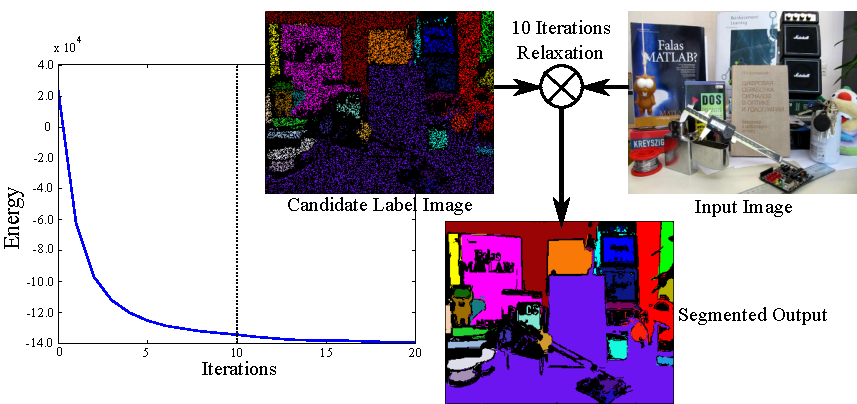
\includegraphics[width=\linewidth]{figures/ECCV2012/ConvergenceFig2.pdf}
\caption[Relaxation Convergence]{The relaxation process causes the energy of the label image to converge after few iterations (outcome after 10 iterations shown here). This results in efficient calculation of an accurate and temporally coherent segmentation.}
\label{fig:Convergence}
\end{figure}

Superparamagnetic clustering of data was chosen due to its flexibility in allowing the use of any initialization state; there are no particular requirements to the initial states of spin variables. The closer the initial states are to the equilibrium, the less time the Metropolis algorithm needs to converge. This property makes it possible to achieve temporal coherency in the segmentation of temporally adjacent frames by using the sparse label configuration taken from the candidate label image for the spin initialization of the current frame. A final (dense) segmentation result is obtained within a small number of Metropolis updates. Conventional segmentation methods do not generally have this property and cannot turn a sparse segmentation prediction into dense final segments which preserve temporal coherence. Moreover, since the method can directly use sparse predictions as the seed of the segmentation kernel, we can avoid the costly and error-prone block-matching procedure required to find label correspondences in other 
work, such as in Brendel and Todorovic \cite{SegTrackRegions} or Hedau et al.  \cite{MatchingUnstable}. Figure \ref{fig:Convergence} illustrates the relaxation process, and the convergence of energy after a small number of iterations. 

\section{Experimental Results}
\label{sec:Experimental Results}

In order to evaluate performance, we compare our method to the state of the art on several challenging video tracking benchmark sequences which are available online\footnote{http://www.GPU4Vision.org}. It should be noted that, as opposed to the other tracking algorithms, we do not pre-select a region to track, and track fully deforming object masks (rather than a rectangle). Additionally, we employ no learned or a-priori specified models, use 50 particles per label, and only have two parameters; the repopulation and decay rates $\lambda_r$ and $\lambda_d$, which were both held constant at $0.05$ throughout testing. Results are compared to the PROST \cite{PROST}, MilTrack \cite{MilTrack}, FragTrack \cite{FragTrack}, and ORF \cite{ORF} tracking algorithms. Further details concerning the parameters used for the above algorithms in the benchmarking can be found in \cite{PROST}.
\begin{table}[!t]
 \caption[PROST dataset benchmark results]{PROST dataset benchmark results. The top table gives average pixel error (lower is better), and the bottom table gives PASCAL based scores (higher is better). Our scores are listed under ``HybridPF''. We compare favorably in three of the sequences, and fail on the ``box'' sequence due to our unsupervised initialization of objects to track. }
\begin{center}
\begin{tabular}{|l|c|c|c|c|c|c|}
\hline
Sequence &  PROST  & MIL & Frag & ORF & HybridPF \\
\hline\hline
Lemming & 25.1 & 14.9 & 82.8 & 166.3 & 19.8\\
Box & 13.0 & 104.6 & 57.4 & 145.4 & 114.1\\
Liquor & 21.5 & 165.1 & 30.7 & 67.3 & 25.5\\
Board & 39.0 & 51.2 & 90.1 & 154.5 & 30.9\\
\hline
\hline
\hline\hline
Lemming & 70.5 & 83.6 & 54.9 & 17.2 & 73.9\\
Box & 90.6 & 24.5 & 61.4 & 28.3 & 7.5\\
Liquor & 85.4 & 20.6 & 79.9 & 53.6 & 54.2\\
Board & 75.0 & 67.9 & 67.9 & 10.0 & 71.4\\
\hline
\end{tabular}
\end{center}
\label{table:results}
\end{table}

We shall not evaluate the visual quality of segmentation results here for a couple of reasons. First, detailed evaluation of the visual quality of super-paramagnetic clustering has been presented in \cite{Abramov_RealtimeSegmentation} in great detail. The visual quality of the segmentation results obtained from this work do not differ significantly from these results, with the exception of labels having continuity through occlusions. Secondly, it is directly acknowledged in other \gls{vos} work that the methods fail under partial \cite{MSVS,PropValAgg} or full \cite{SegTrackRegions,MHVS} occlusions. As such, comparing performance to other \gls{vos} methods is somewhat unreasonable. Rather, the better comparison is to the state of the art in tracking methods, which attempt to handle full and partial occlusions.

In order to compare with the other methods, we needed to output a tracking rectangle for each frame. To do this, once the sequence was segmented, we found the segment which corresponded to the object to track in the first frame, and then took the bounding-box which contained it in each frame as the tracking rectangle. This bounding-box was then compared to ground-truth using two measures; Euclidean distance and the PASCAL-challenge based score proposed in \cite{PROST}. The latter compares the area of intersection of the ground truth and tracked box with the union of the same. When this is greater than 0.5, the object is considered successfully tracked. Table \ref{table:results} gives our results, as well as the results for the other methods.
 
 Testing showed that, when certain assumptions hold, our algorithm performs on par with, and in some cases outperforms, state of the art tracking algorithms. This is the case for the \textit{liquor}, \textit{lemming}, and \textit{board} sequences. In the \textit{lemming} sequence, frames of which are shown in Figure \ref{fig:Results}, our algorithm outperforms the other methods in cases of occlusion, especially when the tracked object is fully occluded. While other methods offer false positives and erroneous tracks, our method decays the label for the object and avoids proposing incorrect tracking solutions. In the \textit{liquor} sequence, our algorithm adapts to the changing appearance (size, shape, and color) of the tracked bottle, allowing it to maintain performance on par with the other algorithms, in spite of the difficulties of segmenting transparent objects. In the \textit{board} sequence, our method successfully adapts to the rapidly changing appearance of the tracked board as it rotates, allowing it to maintain an accurate track and outperform the other methods.

In addition to showing the strengths of our method, a weakness was also highlighted by the benchmark sequences. The \textit{box} sequence demonstrated the limitations of using unsupervised color-based segmentation to initialize the objects to track. In the sequence, the object to track contains strong color differences, which are segmented into different initial regions. As the object moves around, the particles for these regions are attracted to other objects it passes over which have similar color.  

%color histograms as a measurement. In the sequence, the black box being tracked passes in front of another black box several times. In almost all cases, particles are attracted to the other box, which results in twin peaks in $\mathbf{\hat{M}}^k_{t}$. While the tracked object is not lost, this results in the final segmented output having the same label for both boxes.

\begin{figure}[!t]
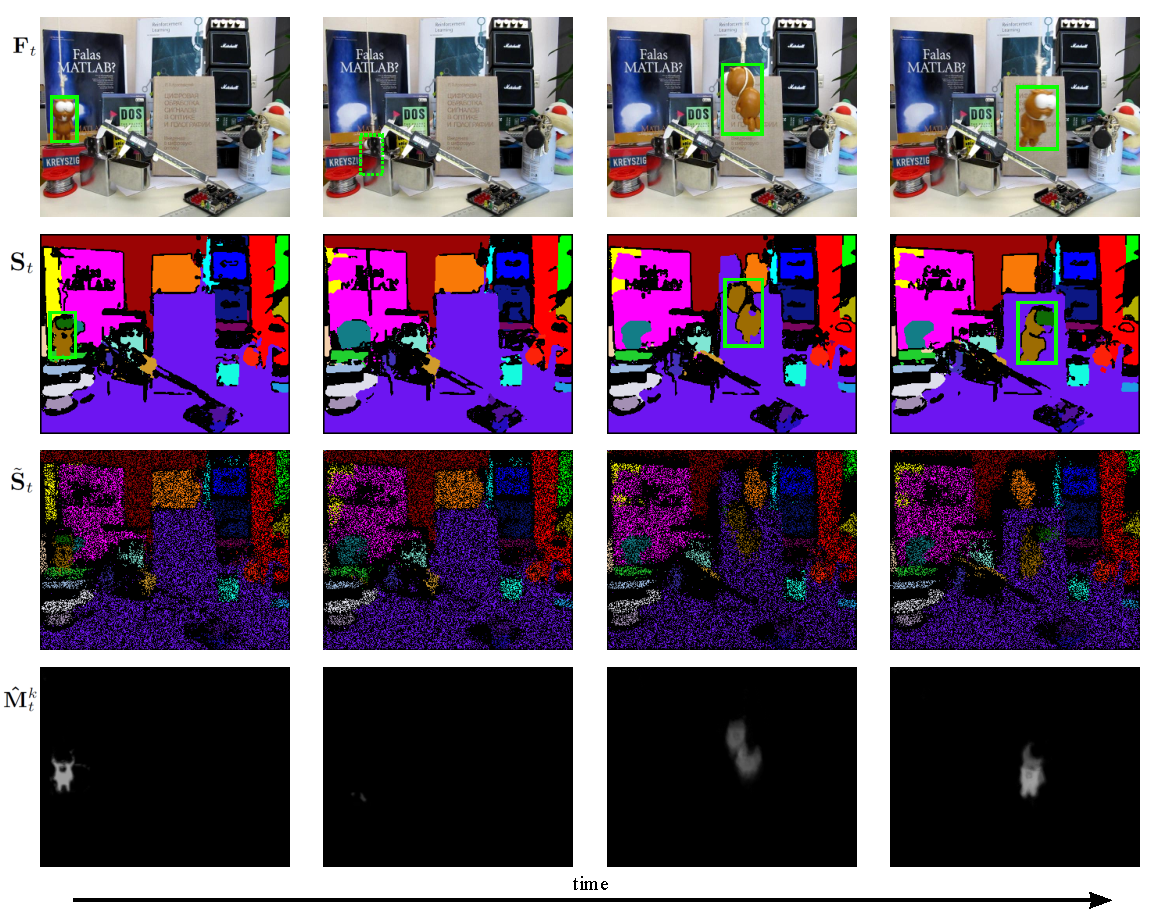
\includegraphics[width=\linewidth]{figures/ECCV2012/Tracking.pdf}
  \caption[Tracked output from lemming sequence]{Output frames from the \textit{lemming} sequence, in which a target is completely occluded (for $\sim20$ frames, second column) and changes significantly in appearance. The object which is tracked for comparison to other algorithms is highlighted with a green box. $\mathbf{F}_t$-Original frames from  movie.~~$\mathbf{S}_t$-The output of the segmentation algorithm.~~$\tilde{\mathbf{S}}_{t}$-The candidate label image constructed by taking a random draw from $\hat{\mathbf{L}}_{t}$, the label association likelihood map.~~$\hat{\mathbf{M}}^k_{t}$-The overall object pixel likelihood map for the lemming label, created by combining the set of particles for the label. Intensity represents the sum of the normalized weights of the set of particles.}
\label{fig:Results}
\end{figure}

\begin{figure}[!t]
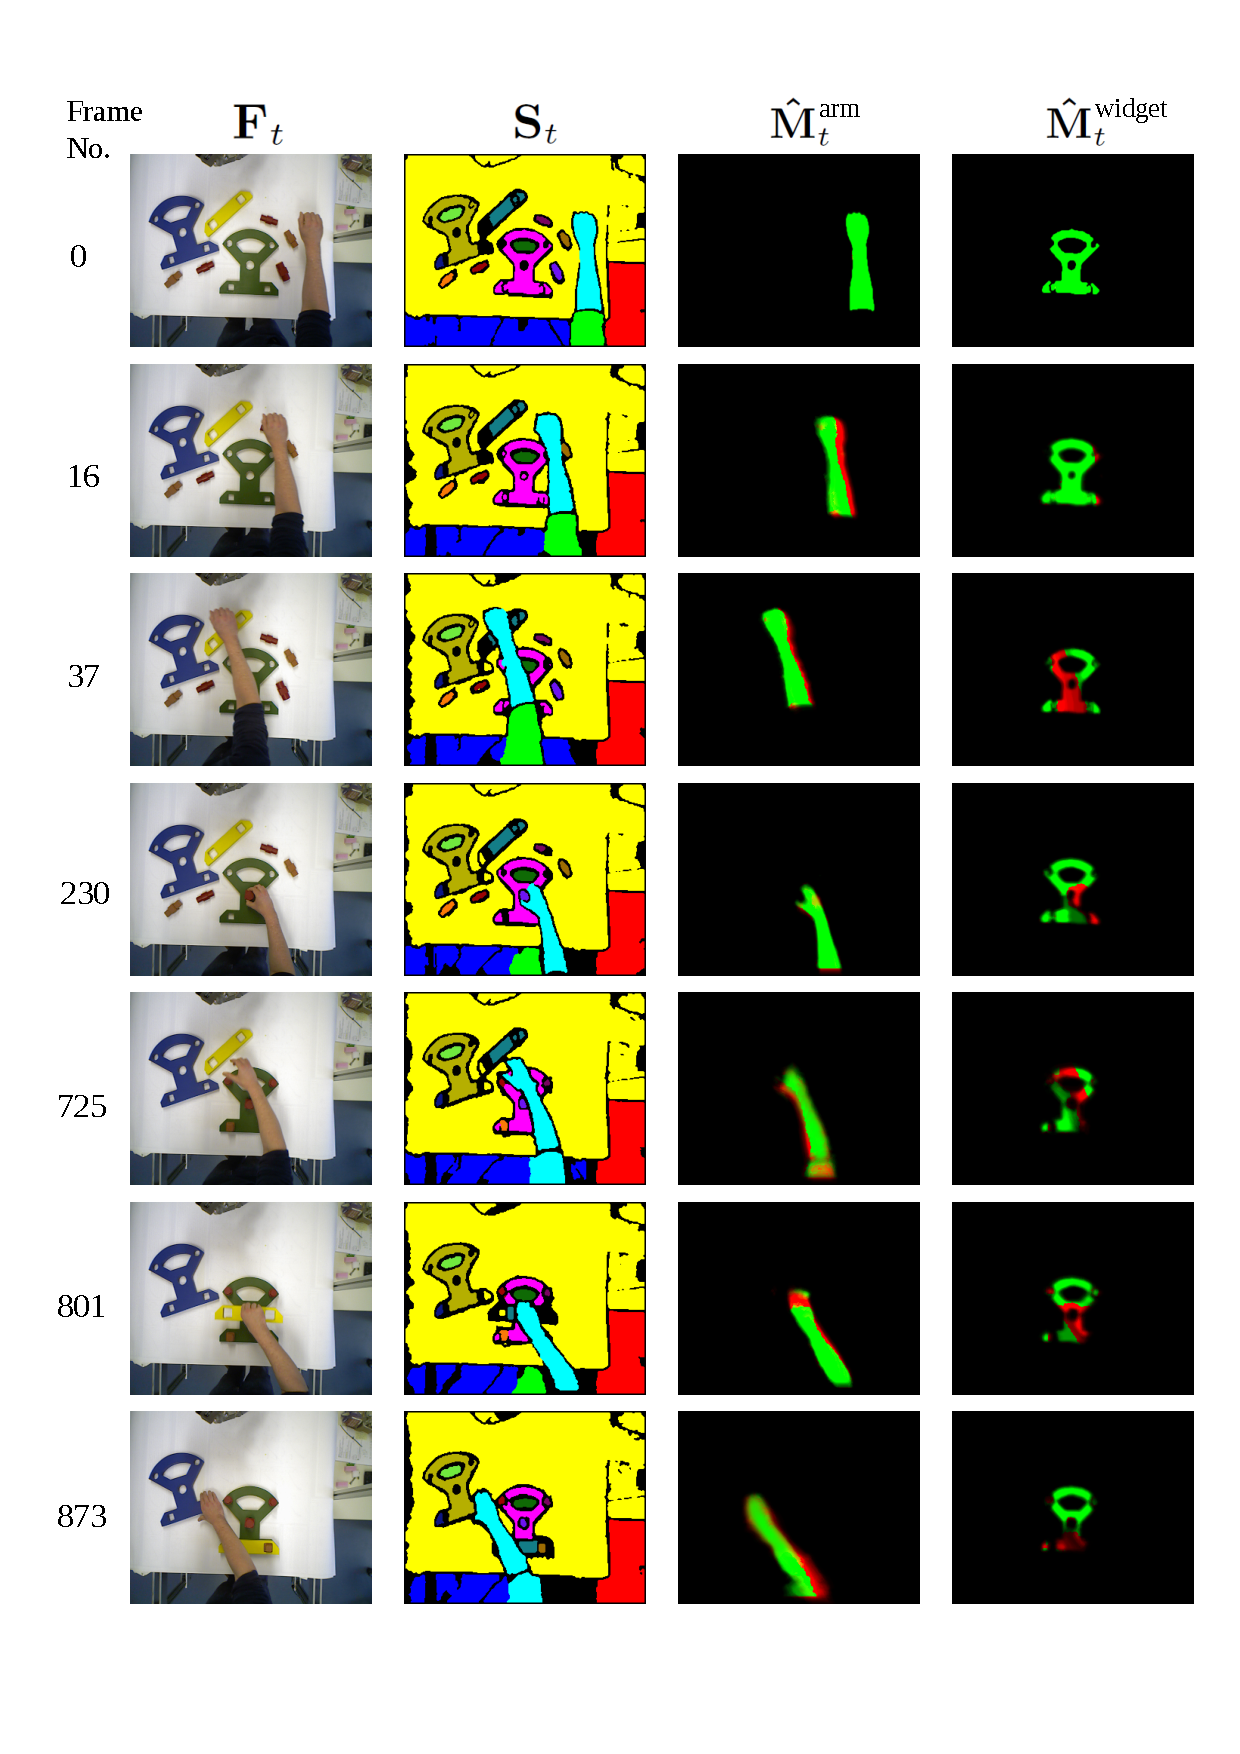
\includegraphics[width=\linewidth]{figures/ECCV2012/Cranfield_Results.pdf}
  \caption[Results of Cranfield Sequence]{Results of segmentation on Cranfield Benchmark Sequence. Green masks show observed pixels, while red masks show occluded pixels which are believed to belong to the object.}
\label{fig:Cranfield_Results}
\end{figure}

\section{Discussion}
In this chapter we presented a new method for performing on-line, dense, unsupervised video segmentation which uses tracking as the basis for segmentation. We have given results which show that the method is able to resolve occlusion relations between objects without explicitly modeling them, and can maintain consistent labels for objects, even when they leave and re-enter the field of view. Additionally, we have shown that the method is able to adapt to rapidly changing appearance of tracked objects, producing consistent segmentations over lengthy video sequences. A GPU version of the algorithm has been developed that can achieve near real-time levels ~10 fps at 640x480 resolution on an i7 standard desktop. The algorithm has significant advantages over other \gls{vos} methods, in particular when it comes to occlusion handling and speed.

Unfortunately, we found that there were significant instabilities in the algorithm that compounded over time. While these instabilities did not show up in the short sequences used to benchmark, if the algorithm was run for several minutes, it would tend to decay into a state where one or two large segments dominate the others. The other tracking algorithms did not suffer from this, as they only tracked single targets. We address this problem of instability in subsequent work by reinitializing the segments periodically and finding a solution to the data-association problem.

Another disadvantage of the method is its vulnerability to situations where objects have similar color distributions. This is an inherent flaw of standard (i.e. color-based) video tracking and segmentation systems - they are unable to use 3D shape to resolve ambiguities. As there are many situations where color is not a useful feature for resolving objects, one must reason about real-world geometry in order to reliably track and segment objects. While it is theoretically possible to infer 3D geometry without depth information, the inference tends be noisy and error-prone, even for the human visual cortex (consider how easy it is to fool one's depth-reasoning with one eye closed). As such, we decided to progress from standard video to RGB-D sensors which provide measured depth information for each pixel, allowing us to incorporate 3D geometry directly into our measurement function and segmentation features. In subsequent Chapters we shall investigate how to take advantage of depth information while remaining efficient, and how to handle point cloud data which lacks the rigid lattice of image data. With this in mind, in the next Chapter we establish a graph-based framework for efficiently representing streaming unstructured point cloud data. 


